\documentclass[12pt, a4paper]{article}


\usepackage[utf8]{inputenc}
\usepackage[english, slovene]{babel}
\usepackage{eurosym}
\usepackage{graphicx}
\usepackage{enumerate}
\usepackage{framed}
\usepackage{mathtools}
\usepackage{amsmath, amsfonts}
\usepackage{xcolor}
\usepackage{esvect}
\usepackage{MnSymbol, wasysym}
\usepackage{tikz}
\usepackage{fancyhdr}

\newcommand{\Q}{\mathbb{Q}}
\newcommand{\al}{\alpha}


\title{Inženirji, matematiki in fiziki}
\author{Klara Golob}
\date{\today}

%\pagenumbering{arabic}
%roman
%alph

\pagestyle{fancy}
\fancyhf{}
\lhead{LaTeX}
\rhead{\thepage}
\chead{Tečaj}

%\cfoot{Poglavje \thesection}



\begin{document}

\begin{titlepage}
\selectlanguage{slovene}
\maketitle

\centering Mentor: Prof. Moj Mentor

\vfill
%\hfill
%\hspace{3cm}
Akademija Strojnik.si
\thispagestyle{empty}
\end{titlepage}

%kazalo
\tableofcontents
\listoffigures
\listoftables

\newpage 

\selectlanguage{slovene}
\begin{abstract}
Matematki, inženirji, fiziki,... vsi delajo na istem področju, a ne enakih stvari. Verjetno eni brez drugih ne bi mogli, a to si teˇzko priznajo, vsaki vedno pravijo, da so oni, tisti ”ta bolj pomembni”. Kdo pa je ”pomembnejˇsi” po vaˇsem mnenju?
\end{abstract}

\selectlanguage{english}
\begin{abstract}
Mathematicians, engineers, physicists,... they all work in the same field, but they don’t do the same job. Probably one couldn’t exist without the other, but still, all say for themselves they are the ones ”who are more important”. Who is ”more important” in your opinion?
\end{abstract}

\vfill
\noindent
{\bf Ključne besede:} diploma, LaTeX, Akademija Strojnik.si \\
{\bf Keywors:} diploma, LaTeX, Akademija Strojnik.si 

\newpage
\null
\newpage

\section{Uvod}
Inˇzenir, fizik in matematik dobijo nalogo, naj najdejo najuˇcinkovitejˇsi naˇcin za gradnjo ograje okrog ˇcrede ovc.

\begin{itemize}
\item Inˇzenir predlaga praktiˇcno reˇsitev: ”Fanta, najbolje bo, da pregledamo razliˇcne vrste ograj in izberemo tisto, ki bo najbolj ustrezna za ˇstevilo ovc, ki jih moramo ograditi, ter obenem tudi najbolj poceni.”
\item Natanˇcni fizik se ne da: ’Se ne strinjam. Najboljˇsi naˇcin je, da zgradimo ograjo z obsegom ekvatorja, nato pa jo skrajˇsujemo, dokler se ne bo dotaknila prve ovce v ˇcredi.’
\item Matematik pa vzame ˇstiri deske, se ogradi z njimi in zmagoslavno izjavi: ”Jaz sem zunaj ograje.”
\end{itemize}

\section{Inženir}

\subsection{Inženir kot zdravnik}
Nek inˇzenir, ˇze dlje ˇcasa brezposeln, se odloˇci da bo odprl ambulanto, ker je denar v zdravstvu dober, pretegnejo se zdravniki ravno ne, posla pa je veˇc kot dovolj. Poglej na sliko \ref{fig:inzenir_zdravnik}. Na znaku nad vhodom je zapisal: \textit{Inˇzenirska ambulanta, ˇce vas ozdravimo, nam plaˇcate 50 \euro, ˇce vas ne ozdravimo – vam mi plačamo 100 \euro.}
\\ \\
\indent
V istem kraju ima ambulanto tudi zdravnik, ki je nekoliko nejevoljen nad inˇzenirjem in njegovo novo ambulanto. Ko gre mimo in prebere napis nad inˇzenirjevo ambulanto, si pomane roki, in z mislijo na lahko zasluˇzenih 100 € vstopi.


\begin{figure}[h]
\centering \includegraphics[width=5cm]{Inzenir_doktor.jpg}
\selectlanguage{slovene}
\caption{Tudi inženir je lahko zdravnik.}
\label{fig:inzenir_zdravnik}
\end{figure}

\subsubsection{Prvič v ordinaciji}

\begin{enumerate}
\item \textbf{Inženir}: Dober dan, kaj vas tare?
\item \textbf{Zdravnik}: Paaa, veste, zdi se mi, kot da ne ˇcutim veˇc okusov . . .
\item \textbf{Inženir}: Sestra, iz predala 22 vzemite zdravilo in ga dajte pacientu 3
kapljice na jezik . . .

\end{enumerate}

Zdravnik ves jezen plaˇca in odide. Ves teden ga je morilo tistih 50\euro, zato se odloˇci, da ponovno obiˇsˇce inˇzenirjevo ambulanto. Prebere napis nad inˇzenirjevo ambulanto, si pomane roki, in z mislijo na lahko zasluˇzenih 100 \euro vstopi.

\subsubsection{Drugič v ordinaciji}

\begin{enumerate}
\item[a.)] \underline{Inženir}: Pozdravljeni ponovno! Kaj vas tokrat tare?
\item[b.)] \underline{Zdravnik}: Veste, se mi zdi da kar izgubljam spomin . . . Enostavne reˇci mi ˇze delajo teˇzave . . . Spomin je slab, ne vem veˇc niti tega, kaj sem vˇceraj jedel . . .
\item[c.)] \underline{Inženir}: Oh, to je ozdravljivo! Sestra, iz predala 22 vzemite zdravilo in ga dajte pacientu 3 kapljice na jezik!
\end{enumerate}

Zdravnik je besen, ker se je spet pustil tako zlahka ofrnaˇziti inˇzenirju.
Ves teden kuha peklenski naˇcrt, kako si vsaj povrniti 100€. Naposled spet obiˇsˇce inˇzenirjevo ambulanto.

\subsubsection{Tretjič v ordinaciji}

\begin{enumerate}[i]
\item \textit{\textbf{Inženir}}: Pozdravljeni, Vi ste pa ˇze skoraj moja stalna stranka! Kako Vam lahko pomagam?
\item \textit{\textbf{Zdravnik}}: Veste, vid mi peˇsa. Najprej so ˇsli detajli, sedaj vidim le ˇse obrise ob moˇcni svetlobi, v senci sem praktiˇcno slep . . .

\end{enumerate}

\subsubsection{Stanje}

Finančno stanje obeh je prikazano v tabeli \ref{tab:tabela}.

\begin{table}[h!]
\centering
\begin{tabular}{r | r | r | r | r}
 & 1.dan & 2.dan & 3.dan & \textbf{skupaj} \\ \hline
 inženir & 50 & 50 & 50 & 150 \\ 
 Zdravnik & -50 & -50 & -50 & -150 \\ 
\end{tabular}
\selectlanguage{slovene}
\caption{Tabela}
\label{tab:tabela}
\end{table}

\begin{figure}[h]
\includegraphics[width=6.5cm]{inzenir.jpg}
\ \ \ 
\includegraphics[width=6.5cm]{doktor.jpg}
\selectlanguage{slovene}
\caption{Inženir in doktor.}

\end{figure}

\section{Matematiki}

Kaj matematika najbolj razburi?\footnotemark
\footnotetext{Tudi najkrajši matematični vic.}

\begin{framed}
$$  \epsilon < 0 $$
\end{framed}

\subsection{Najlepše matematične formule}
\subsubsection{Riemannova zeta funkcija}

\begin{equation}
\zeta (s) = \sum_{n=1}^{\infty} \frac{1}{n^s} = \frac{1}{1^s} + \frac{1}{2^s} + \frac{1}{3^s} + \cdots
\end{equation}

\subsubsection{Einsteinove enaˇcbe polja}

\begin{equation}
R_{ab} = \frac{1}{2}Rg_{ab} = -\kappa T_{ab},
\end{equation}
kjer je konstanta

\begin{equation}
\kappa = -\frac{8\pi G}{c^4} \approx 2{,}077 \times 10^{-43} N^{-1}.
\end{equation}

\subsubsection{Drugi osnovni izrek infinitezimalnega raˇcuna}

$$ \int_{a}^{b} f(\alpha)d\alpha = F(\alpha) \bigg |_{a}^{b} = F(b) - F(a). $$

\subsubsection{Integriranje parcialnih ulomkov}

\begin{equation}
\int \left(\frac{Bx+C}{x^2+bx+c}\right)dx = \frac{B}{2} \ln |x^2 + bx +c | + \frac{2C-Bb}{\sqrt{-D}} \arctan \left[ \frac{2x+b}{\sqrt{-D}} \right] + E,
\end{equation}

\textbf{kjer predpostavimo, da je} $D = b^2-4c < 0.$

\subsubsection{Funkcija, ki nima določen integral}

\begin{equation*}
f(x) = 
\begin{cases}
	1, x \in [0, 1] \cap \Q, \\
	0, x \in [0, 1] \backslash \Q .
	\end{cases}
\end{equation*}

\subsubsection{Sistem linearnih enačb}

\begin{gather} \label{prva_enacba}
x+y+z = 6, \\ \label{druga_enačba}
2y+5z = -4, \\ \label{tretja_enačba} 
2x+5y-z = 27.
\end{gather}

Enačbe \eqref{prva_enacba}, \eqref{druga_enačba} in \eqref{tretja_enačba} lahko zapišemo v magtrične enačbe:

\begin{equation*}
\begin{bmatrix}
1 & 1 & 1 \\
0 & 2 & 5 \\
2 & 5 & -1
\end{bmatrix}
\begin{bmatrix}
x \\
y \\
z
\end{bmatrix}
=
\begin{bmatrix}
6 \\
-4 \\
27
\end{bmatrix}
\end{equation*}

\subsection{Koliko matematikov potebujeˇs, da zamenjajo ˇzarnico?}

Odvisno od njihove specializacije!

\begin{itemize}
\item \textit{Koliko profesorjev matematike potebujeˇs, da zamenjajo ˇzarnico?}
\begin{itemize}
\item \underline{\textbf{Nič}}. To vedno pustijo uˇcencem za domaˇco nalogo.
\end{itemize}
\item \textit{Koliko numeriˇcnih matematikov potebujeˇs, da zamenjajo ˇzarnico?}
\begin{itemize}
\item \underline{\textbf{1{,}99521}} Pribliˇzek po petih korakih iteracije.
\end{itemize}
\end{itemize}

\section{Fiziki}
\subsection{Skrivalnice}

\textcolor{red}{Albert Einstein}, \textcolor{blue}{Isaac Newton} in \textcolor{brown}{Blaise Pascal} se igrajo skrivalnice. Prvi do deset ˇsteje Einstein. Pascal se skrije, Newton pa na tla nariˇse kvadrat s strani- cami, dolgimi en meter, in stopi nanj. Einstein ga takoj vidi in zmagoslavno izjavi: \colorbox{pink}{”Newton, naˇsel sem te!”} Newton odvrne: \colorbox{green}{\underline{\underline{”Ne, naˇsel si Pascala.”}}}

\section{Polet z balonom}

\begin{framed}
Inˇzenirja in fizika med poletom z balonom na vroˇc zrak ujame veter in odnese daleˇc s poti. Ker ne vesta veˇc, kje sta, inˇzenir v upanju, da ga bo kdo sliˇsal, zaˇcne kriˇcati: ”Na pomoˇc! Ali nama lahko kdo tam
ˇ
spodaj pove, kje sva?” Ce nekaj ur zasliˇsita glas: ”V balonu na vroˇc
zrak”. Fizik reˇce inˇzenirju: ”Ta ˇclovek je bil zagotovo matematik. Po urah razmisleka nama je dal odgovor, ki je sicer povsem pravilen, a tudi popolnoma neuporaben.”
\end{framed}

\subsection{Svetloba}

\begin{align*}
&\nabla \cdot \vv{D} = \rho_{free}, \\
&\nabla \cdot \vv{B} = 0, \\
&\nabla \times \vv{E} = - \frac{\partial \vv{B}}{\partial t}, \\
&\nabla \times \vv{H} = \vv{J}_{free} + \frac{\partial \vv{D}}{\partial t},
\end{align*}
 
in potem je bila svetloba. \smiley{}

\section{Rezultati}

V bistvu ni vaˇzno kdo je kdo. Vsak ima svoje fore, svoje prednosti in slabosti. Kakor pa ˇze na zaˇcetku povedano, eni brez drugih ne bi mogli. Zato za enkrat ostanimo le pri ˇsalah.


\begin{center}
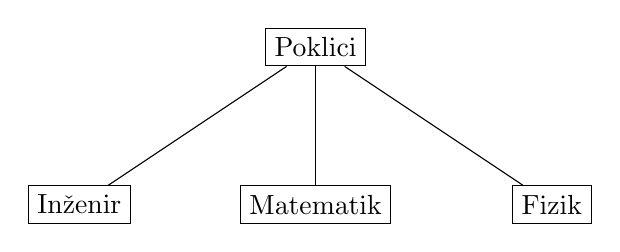
\begin{tikzpicture}[every node/.style={draw}]
\node (a1) at (3,3){Poklici};
\node (a2) at (3,1){Matematik};
\node (a3) at (0,1){Inženir};
\node (a4) at (6,1){Fizik};

\draw (a1) -- (a3);
\draw (a1) -- (a2);
\draw (a1) -- (a4);
\end{tikzpicture}
\end{center}

\section{Zaključek}

V zakljuˇcku si bomo pogledali ˇse, kako se na koncu vstavi literaturo, ki sicer v naˇsem primeru ni vezana na vsebino. Poglejmo si primere \cite{vidav}, \cite{article1} in \cite{article2}

\selectlanguage{slovene}
\bibliographystyle{unsrt}
\bibliography{literatura}













\end{document}